  
  \frame{
  \frametitle {Our first simple Docker image}
 To create our image we will perform the following tasks:\vspace{0.4cm}
 \begin{itemize}
 \item Create an own docker public repository;\vspace{0.2cm}	
 \item Download a  base image from the Docker Hub;\vspace{0.2cm}	
 \item Updating the download image and upload it on our own repository;\vspace{0.2cm}	
 \item Create and embed  simple BASH and R  scripts on our image;\vspace{0.2cm}	
 \item Execute the new created image.
 \end{itemize}
}
  
    \frame{
  \frametitle {Our first simple Docker image}
 To create our image we will perform the following tasks:\vspace{0.4cm}
 \begin{itemize}
 \item Create an own docker public repository;\vspace{0.2cm}\color{grey}	
 \item Download a  base image from the Docker Hub;\vspace{0.2cm}	
 \item Updating the download image and upload it on our own repository;\vspace{0.2cm}	
 \item Create and embed  simple BASH and R  scripts on our image;\vspace{0.2cm}	
 \item Execute the new created image.
 \end{itemize}
} 
 
  
   \frame{
  \frametitle { Create an own docker public repository}
  We have to create a free \textbf{\color{NavyBlue}docker ID} at the following address: \color{NavyBlue}\url{ https://hub.docker.com/}
  
       	\begin{center}
  			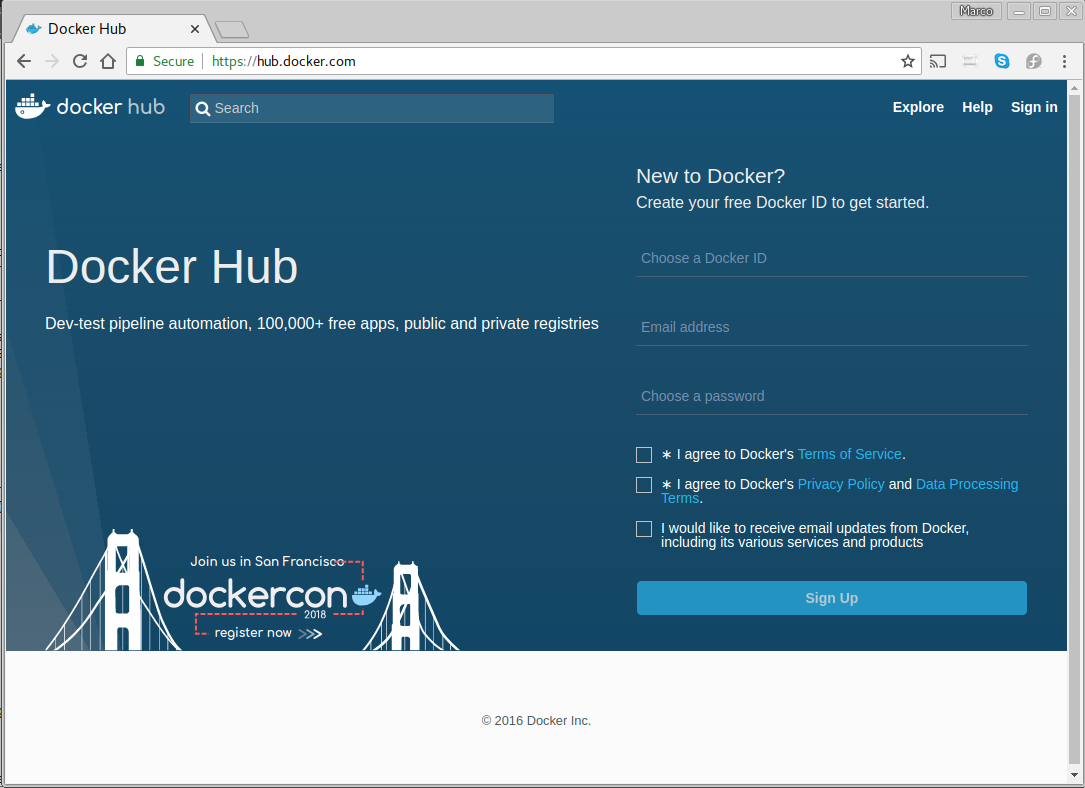
\includegraphics[width=0.60\columnwidth]{./Figure/dockerhub}
  		\end{center}  
  
  
  
  }
    
   \frame{
  \frametitle { Create an own docker public repository}
  We have to create a  \textbf{\color{NavyBlue}public repository} 
  
       	\begin{center}
  			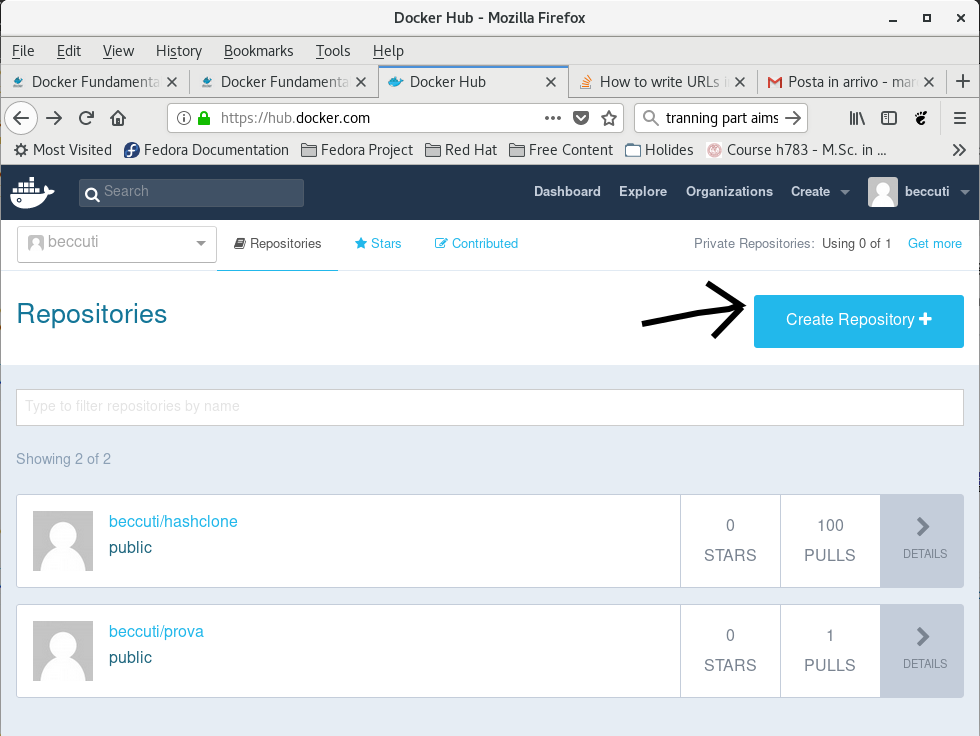
\includegraphics[width=0.60\columnwidth]{./Figure/dockerhub1}
  		\end{center}  
  }
  
    
     \frame{
  \frametitle { Create an own docker public repository}\vspace{0.2cm}
  We have to create a  \textbf{\color{NavyBlue}public repository} 
  
       	\begin{center}
  			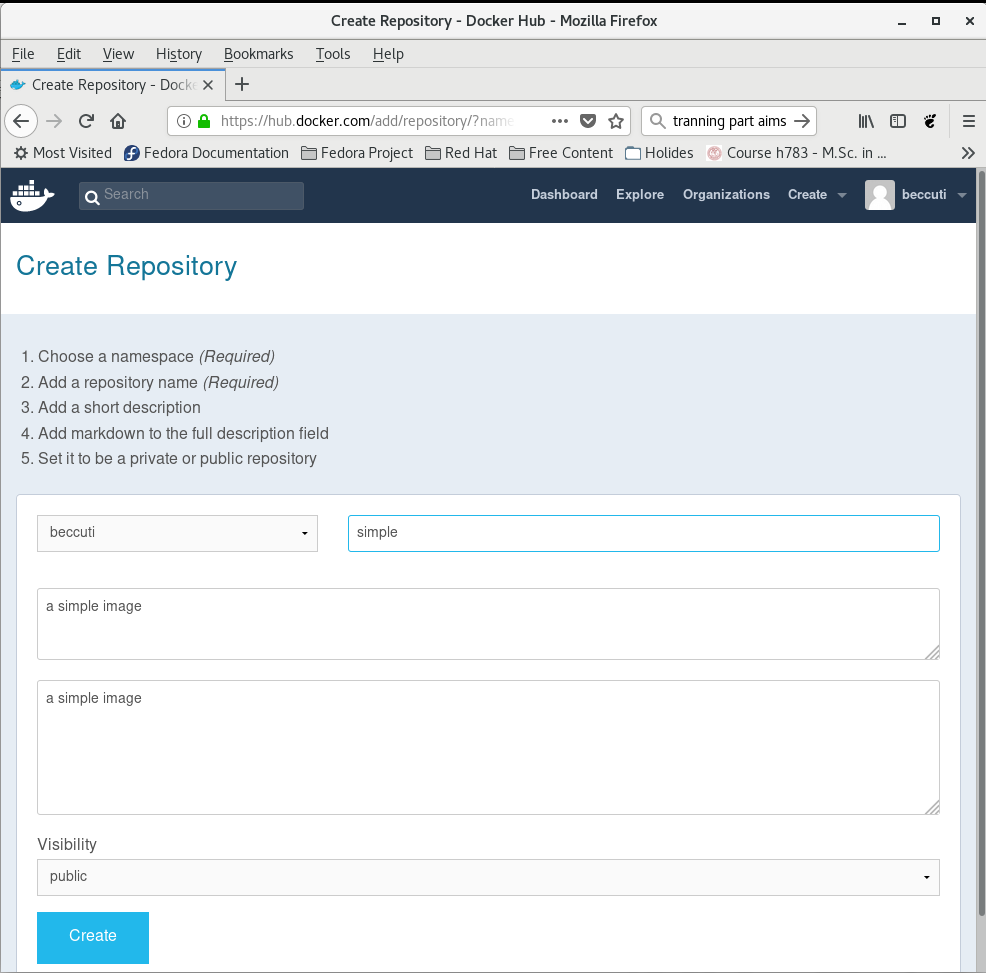
\includegraphics[width=0.63\columnwidth]{./Figure/dockerhub2}
  		\end{center}  
  
  
  
  }
  
       \frame{
  \frametitle { Create an own docker public repository}
  \begin{itemize}
  \item Collaborators can be added;\vspace{0.2cm}
  \item Image id is: \emph{\color{NavyBlue}$\langle$docker\_ID$\rangle$/$\langle$image\_ID$\rangle$} 
  \end{itemize}
       	\begin{center}
  			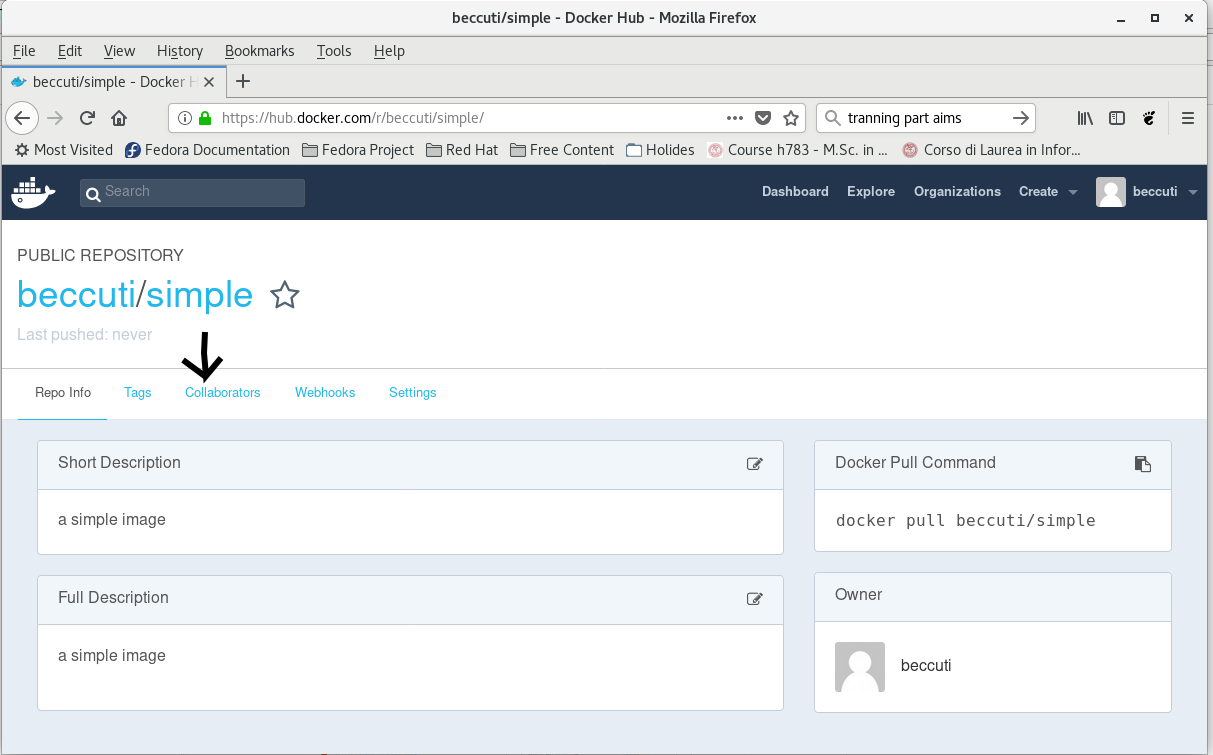
\includegraphics[width=0.85\columnwidth]{./Figure/dockerhub3}
  		\end{center}  
  }
  
 
  \frame{
  \frametitle {Our first simple Docker image}
 To create our image we will perform the following tasks:\vspace{0.4cm}
 \begin{itemize}
 \item Create an own docker public repository;\vspace{0.2cm}
 \item Download a  base image from the Docker Hub;\vspace{0.2cm}	\color{grey}	
 \item Updating the download images and upload it on our own repository;\vspace{0.2cm}	
 \item Create and embed  simple BASH and R  scripts on our image;\vspace{0.2cm}	
 \item Execute the new created image.
 \end{itemize}
} 


   \frame{
  \frametitle {Download a  base image from the Docker Hub}
  We can access the docker documentation at following address: \color{NavyBlue}\url{https://docs.docker.com/}
  
       	\begin{center}
  			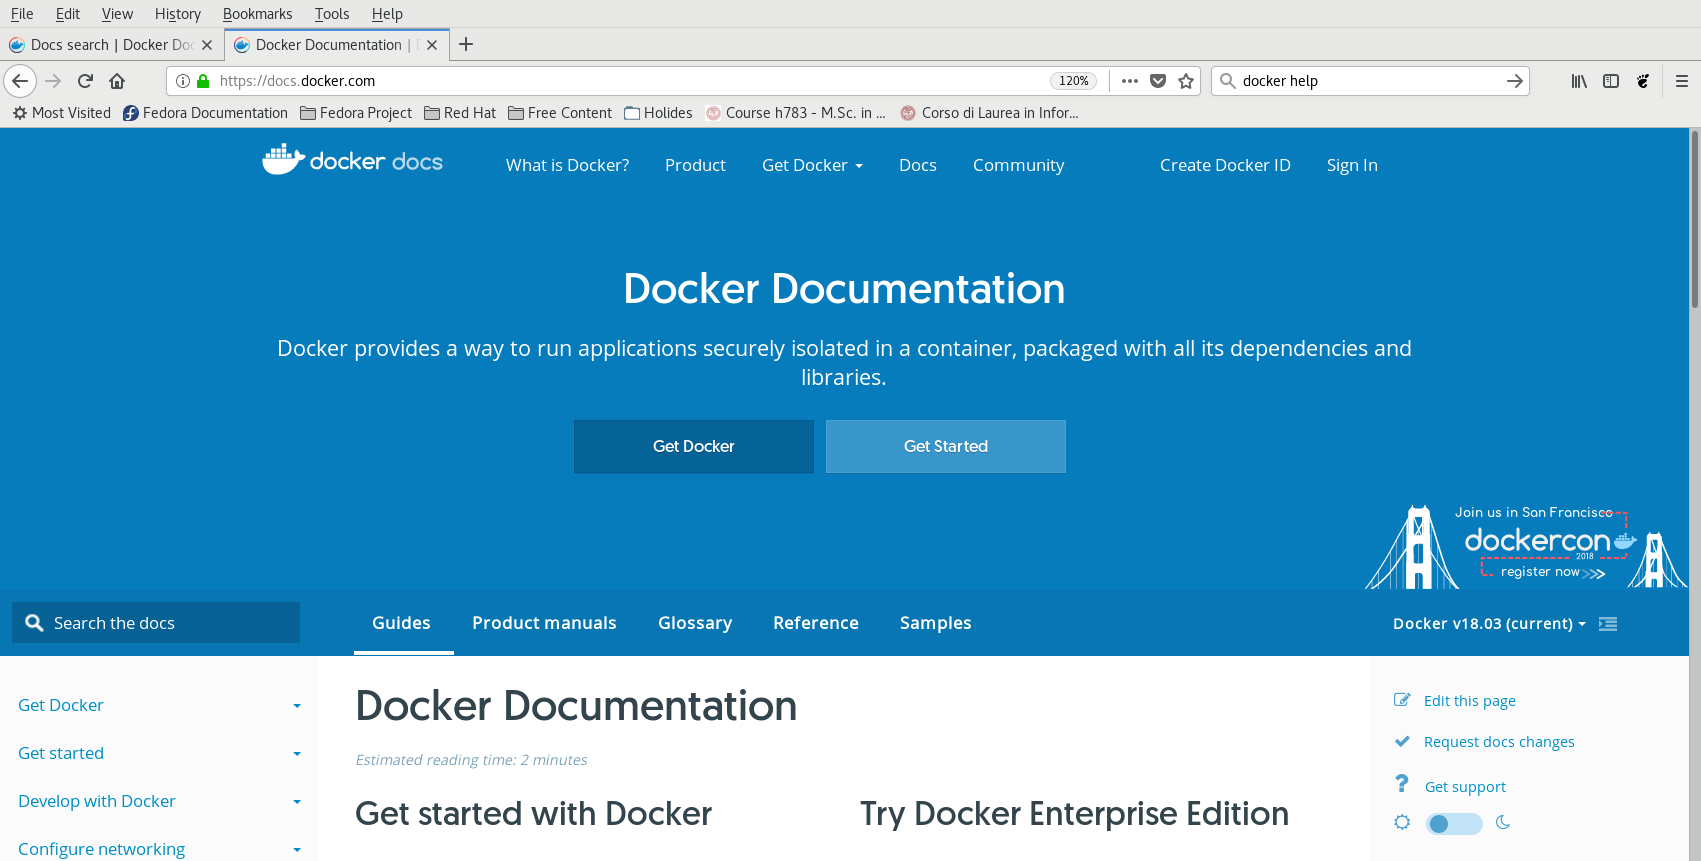
\includegraphics[width=1.00\columnwidth]{./Figure/dockerDoc}
  		\end{center}  
  
  
  
  }
 
  \frame{
  \frametitle {Download a  base image from the Docker Hub}  
 \emph{\color{PineGreen} docker pull 
 $\langle \it{image} \rangle$} can be used to download a docker image from  a hub.
     	\begin{center}
  			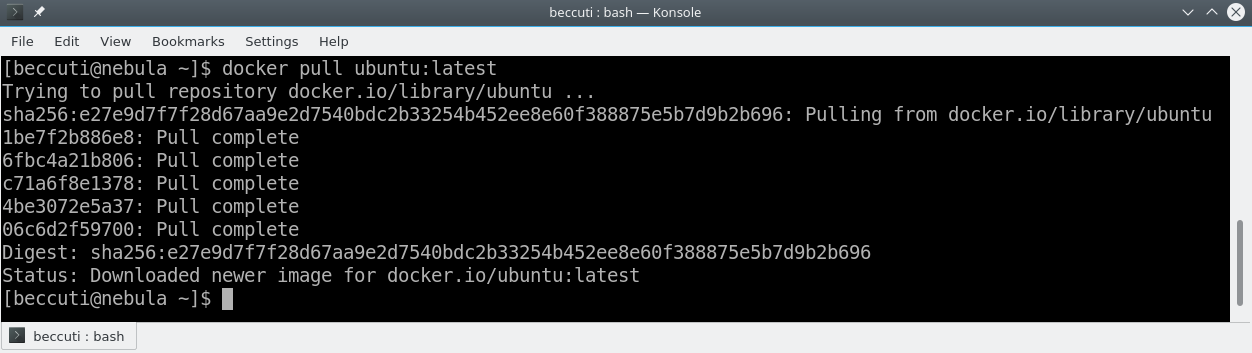
\includegraphics[width=1.00\columnwidth]{./Figure/pull}
  		\end{center}  
 \begin{itemize}
 \item  tags (i.e. \emph{\color{NavyBlue}:$\langle$tag\_name$\rangle$}) can be exploited to choice among different image releases;\vspace{0.2cm}
 \item different releases can \textbf{\color{NavyBlue}share layers} (common image portions) to save disk space;\vspace{0.2cm}
 \item  If no tag is provided, Docker Engine uses the  \emph{\color{NavyBlue}:latest} tag as a default.
 \end{itemize} 
  
 }
 
 
     \frame{
\frametitle{Download a  base image from the Docker Hub} 
  
 \emph{\color{PineGreen} docker images} can be used to list the Docker images installed on a machine. 
     	\begin{center}
  			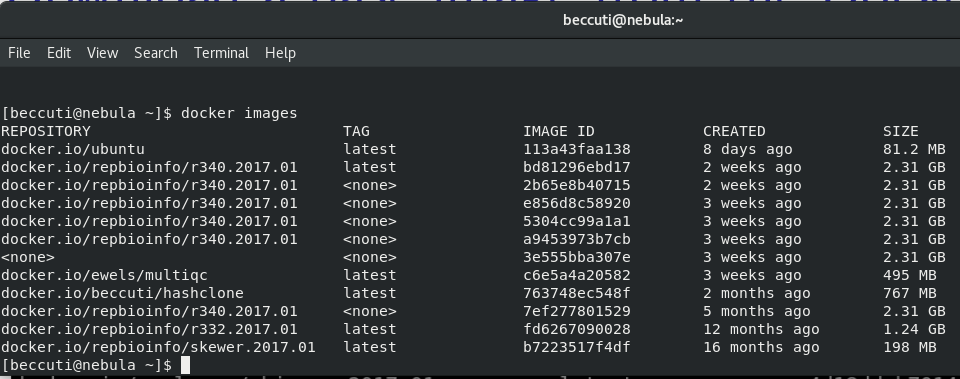
\includegraphics[width=1.00\columnwidth]{./Figure/dockerimages}
  		\end{center}  
  \begin{itemize}
  \item \emph{\color{NavyBlue} <none>:<none>} images are the dangling images which may cause disk space problems;
  \vspace{0.2cm}
  \item Docker does not have an automatic garbage collection system as of now;
   
  \end{itemize}
 }
 
       \frame{
\frametitle{Download a  base image from the Docker Hub} 
  
 \emph{\color{PineGreen} docker rmi 
 $\langle \it{image} \rangle$} can be used to remove a docker image.
     	\begin{center}
  			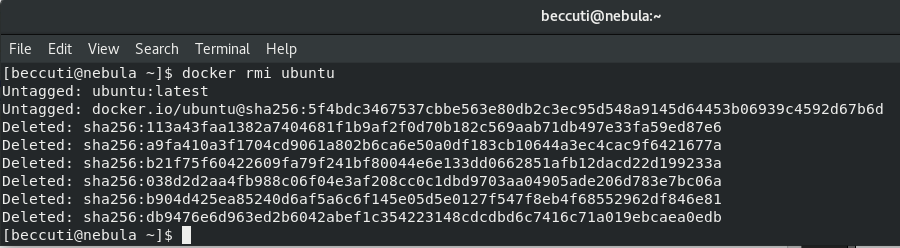
\includegraphics[width=0.97\columnwidth]{./Figure/rm}
  		\end{center}  
  
All \emph{\color{NavyBlue}dangling images} can be removed combining the following two docker commands: 	
 
      	\begin{center}
  			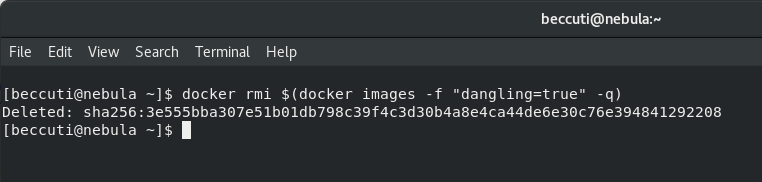
\includegraphics[width=0.97\columnwidth]{./Figure/rm1}
  		\end{center} \vspace{-0.1cm}
 where option \emph{\color{PineGreen}-f "dangling=true"} filters  all the dangling images  and \emph{\color{PineGreen} -q}   returns only docker id.		
 } 	 	
 
       \frame{
\frametitle{Download a  base image from the Docker Hub}  
 	If an image has one or more dependencies, you must remove all of them before.
       	\begin{center}
  			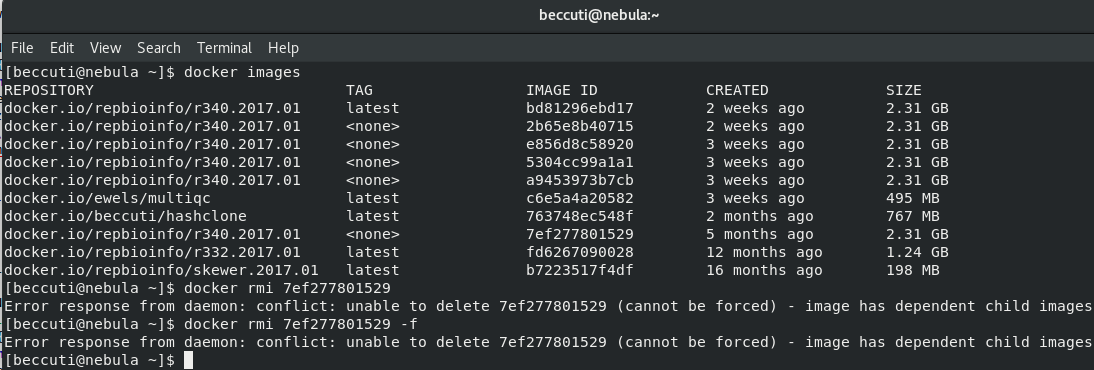
\includegraphics[width=1.02\columnwidth]{./Figure/rm2}
  		\end{center}
}  		

       \frame{
\frametitle{Download a  base image from the Docker Hub}    		
 \emph{\color{PineGreen} docker image history} can be used to list the history of Docker image.  		
        	\begin{center}
  			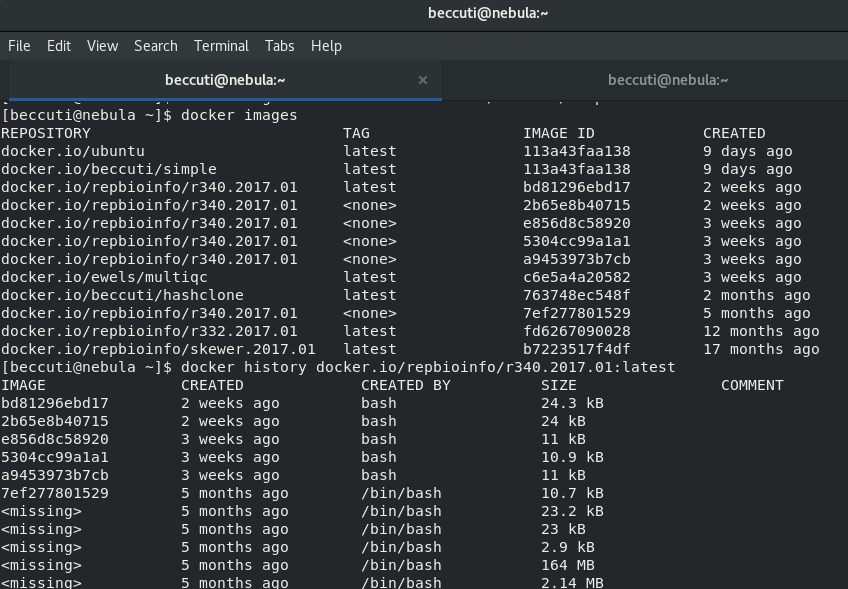
\includegraphics[width=0.90\columnwidth]{./Figure/history}
  		\end{center}%\vspace{-0.2cm}
 Observe that  \textbf{\color{NavyBlue} missing} is for no local dependencies. 		
}  		
  